% \noindent\begin{figure}[htb]
% \centering
% \begin{minipage}[b]{0.5\textwidth}
% 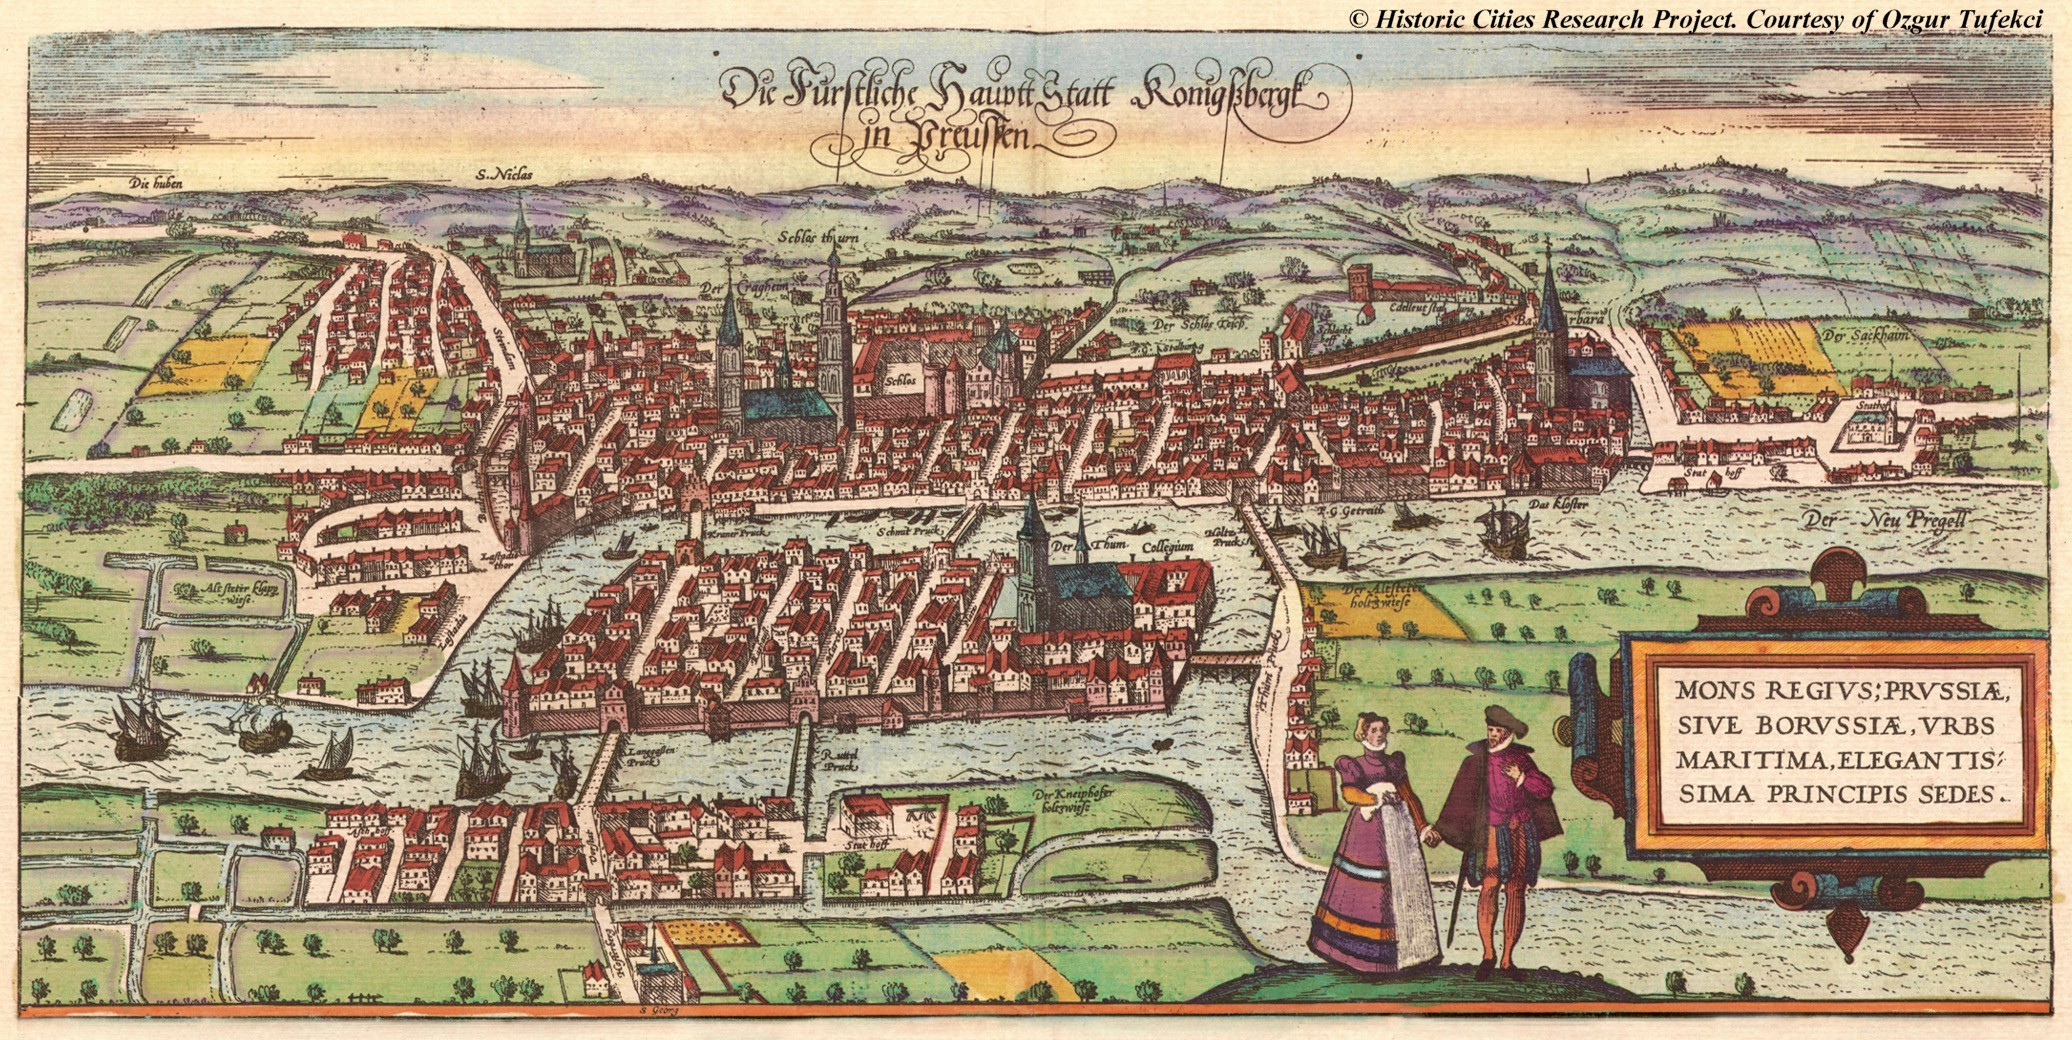
\includegraphics[width=1\linewidth]{images/konigsberg.jpg}
% \end{minipage}\begin{minipage}[b]{0.5\textwidth}
% \centering
% \begin{tikzpicture}
%     \tikzset{LabelStyle/.style= {draw}}
%     \GraphInit[vstyle=Normal]
%     \node[VertexStyle](A){a};
%     \node[VertexStyle,right=of A](B){b};
%     \node[VertexStyle,right=of B](C){c};
%     \node[VertexStyle,above= 1.2cm of B](D){d};
%     \draw[EdgeStyle](B) to node[LabelStyle]{} (D);
%     \tikzset{EdgeStyle/.append style = {bend left}}
%     \draw[EdgeStyle](A) to node[LabelStyle]{} (B);
%     \draw[EdgeStyle](B) to node[LabelStyle]{} (A);
%     \draw[EdgeStyle](B) to node[LabelStyle]{} (C);
%     \draw[EdgeStyle](C) to node[LabelStyle]{} (B);
%     \draw[EdgeStyle](A) to node[LabelStyle]{} (D);
%     \draw[EdgeStyle](D) to node[LabelStyle]{} (C);
% \end{tikzpicture}
% \end{minipage}
% \caption*{\textsf{The city of K{\"o}nigsberg in an old postcard with its graph-theoretical representation, where the bridges are the edges of the graph and the city parts are represented by nodes. This city inspired Euler to start graph theory.}}
% \end{figure}

The methods of network theory date back to the problem of K{\"o}nigsberg bridges, in 1735, when the famous mathematician Leonhard Euler was faced with the problem of finding a path through the city that would cross all the seven bridges just once.
Since then a large amount of knowledge has been accumulated on networks, in what is nowadays known as graph-theory.

Simple graphs are usually defined as a set of nodes, entities representative of some object, connected by a set of links, denoting the strength of the relation between pairs of nodes.
Graphs can be used to represent any type of relation between interacting elements and the idea that graph-theory can be applied to brain networks has been pioneered first by the seminal papers of Olaf Sporns in 2004~\cite{Sporns2004}. In the framework of networks neuroscience, the nodes of graphs typically correspond to anatomically defined brain regions and the links to a measure of interregional interaction or similarity~\cite{bullmore2009}.

For example, in resting state functional connectivity networks, link weights are defined as interregional temporal correlations in the fluctuations of the BOLD signals, and the resulting graph can be represented by a matrix where the strongest correlations indicate the presence of a link between any two specific areas.
Other applications of graph-theory in neuroscience see the links as directly proportional to the number of white matter tracts connecting any two regions.
Additionally, brain networks have also been defined on the basis of inter-subject anatomical covariance~\cite{Evans2013}, co-activation of different brain regions across individuals subjected to experimental tasks~\cite{crossley2013a} or pharmacological challenges~\cite{Schwarz2007,schwarz2008}.
All of these networks are ``weighted'' by definition, i.e. their links are associated with real numbers representing a measure of the strength of pairwise interactions between nodes. 

Across the many properties that graphs exhibit and that are arguments of further analysis per se, one of the most directly observable is that, nodes group together forming some kind of \emph{clusters}.
At this level of meso-scale organization, the topological properties of nodes are more dependent on their neighborhood than on the rest of the graph. When the mesoscopic structure tends to group nodes with similar properties, the meso-scale structure is called \emph{assortative}. Such graphs with assortative structures display consist in tightly connected groups of nodes that are themselves loosely connected with other groups. These groups are therefore dubbed as \emph{communities}. The study of \emph{community} \emph{structure} is \emph{grosso} \emph{modo} the topic of this introductory chapter.
\bigbreak
The community structure is one of the most studied properties of networks: a large amount of literature has grown on community detection, as proved by the one hundred pages of the relatively recent review of Fortunato~\cite{fortunato2010}.
The problem of detecting the communities, or ``graph-partitioning'' in the computer-science jargon, is of big theoretical and practical importance.
From the theoretic point of view, communities in networks are representative of the generative probabilistic model underlying the formation of links~\cite{Karrer2011} and tell much about the statistical properties of the networks.
On the other side, practical applications of community detection are fundamental in sociology, computer science, biology and especially in neuroscience.

%The computational and theoretical models of brain as a graph are being some of the most important subjects of research in complex networks.
It's being increasingly understood indeed, that like many other information processing systems, the brain exhibit a modular architecture.
Within the modules the information is processed locally and is then shared between modules on a communication backbone.\todo{mettere citazione, frase ambigua}
Additionally, the modular organization is exhibited hierarchically at different scales, with modules inside modules, a construction that is thought to confer robustness and adaptability to the network. This kind of structure implies that modules of heterogeneous size are present at the same time in the brain networks and that an efficient method to detect the presence of large and small modules at the same time together is in order.


%Here, we present only two, from the pletora of examples that take advantage of the application of community detection.
%In sociology, the definition of social cliques is important to identify sets of persons with some social relation~\cite{alba1973}. The social-network LinkedIn, in fact, applies community detection as a recommendation system to suggest new friends to the users.
%Biology is extremely rich of examples where community detection plays an important role. The definition of molecular complexes that take part to the same metabolic pathway and that have the similar functions within the cell is expressed as community detection on the graph of protein-protein interaction.

Before delving into the details of community detection, a short introduction to the methods and the jargon of graph-theory is in order.
In Section~\ref{sec:elementsofgraphtheory} we introduce the mathematical concepts of graph theory. In Section~\ref{sec:communitydetectioninnetworks}, we present the problem of community detection in networks. We discuss the main issue of community detection, namely the resolution limit in~\ref{sec:resolutionlimit}. Finally, Surprise, an approach that mitigates the resolution limit is analyzed in deep in section~\ref{sec:surprise}. Different applications of community detection based on Surprise will be then the argument of the next chapters.

This introductory chapter ends discussing the potential methodological improvements that this work may benefit in future.


\section{Elements of graph theory}\label{sec:elementsofgraphtheory}
A short introduction to the basic mathematical terminology of graph theory is given in the following paragraphs. Here we adopt the typical notation used in other works of the network science field~\cite{newman2010book,Estrada2011}.

A \emph{graph} $G=(V,E)$ is a representation of a set $V$ of $n$ nodes, also called \emph{vertices}, connected by $m$ links (or edges), in a set $E$ (Figure~\ref{fig:graphmodelsa}).
One and only one link can exist between two nodes (no \emph{multiedges}), and no links have the same source and target node (no self-loops) as in Figure~\ref{fig:graphmodelsc}.
Graphs with no multiple links and no self-loops are dubbed \emph{simple graphs}.
In the next pages we only consider \emph{undirected graphs}, since we are not interested in the direction of link between two nodes.

The adjacency matrix $\mathbf{A}=\{a_{ij}\} \in \{0,1\}^{n \times n}$ of a binary (undirected) graph is a square $n\times n$ symmetric matrix with elements $a_{ij}=1$ when an edge exists between vertex $i$ and $j$ and $0$ otherwise.

An \emph{edge-weighted graph} (also called weighted graph) $G=(V,E,\omega)$ is a graph that has a set of weights $\omega$ on the links (Figure~\ref{fig:graphmodelsb}). Although not true in general, we consider only weighted undirected graphs with symmetrical real adjacency matrix, meaning that if an edge exists between node $i$ and $j$ the weight from $i$ to $j$ is the same as the weight from $j$ to $i$: $\omega_{ij}=\omega_{ji}$. The weighted adjacency matrix,  indicated as $\mathbf{W}=\{ \omega_{ij} \} \in \mathbb{R}^{n\times n}$ is a real, square $n \times n$ symmetric matrix.

% \noindent\begin{figure}[htb]
% 	\begin{subfigure}[b]{0.25\textwidth}\flushleft
% 		\includegraphics[width=1.0\textwidth]{standalonetikz/tikz_simple_graph.tikz}
% 		\caption{}
% 		\label{fig:graphmodelsa}
% 	\end{subfigure}%
% 	\begin{subfigure}[b]{0.25\textwidth}\centering
% 	\includegraphics[width=1.0\textwidth]{standalonetikz/tikz_weighted_graph.tikz}
% 	\caption{}
% 	\label{fig:graphmodelsb}
% 	\end{subfigure}
% 	\begin{subfigure}[b]{0.25\textwidth}\flushright
% 	\includegraphics[width=1.0\textwidth]{standalonetikz/tikz_loopy_multigraph.tikz}
% 	\caption{}
% 	\label{fig:graphmodelsc}
% 	\end{subfigure}%
% 	\begin{subfigure}[b]{0.25\textwidth}
% 	\includegraphics[width=1.0\textwidth]{standalonetikz/tikz_degree_strength.tikz}
% 	\caption{}
% 	\label{fig:degreestrength}
% 	\end{subfigure}
% 	\caption{Classes of graphs.}
% \end{figure}

The simplest property of the graph, once defined nodes and edges, is the \emph{density} $\rho$. It is defined on a simple graph as the ratio of the number of edges over all possible edges:
\begin{equation}
\rho = \frac{m}{\binom{n}{2}} = \frac{2m}{n(n-1)}.
\end{equation}
A \emph{dense} graph is a graph where almost every possible pair of nodes is connected with an edge. Conversely, a graph is termed \emph{sparse} if the density is low, meaning that also the adjacency matrix is sparse and the number of edges has the order of magnitude of the number nodes $m ~\approx \mathcal{O}(n)$.

The number of edges incident to a node in a simple graph is called \emph{degree}, denoted as $k_i$ (Figure~\ref{fig:degreestrength}). Every half edge incident to a node is called \emph{stub}. A vertex with degree $k_i$ has therefore $k_i$ stubs.
On simple weighted graphs, the sum of weights of the edges incident to a vertex $i$ is called \emph{strength} and is denoted as $s_i$. 
In matrix terms, degree and strength are the sums over rows of the adjacency matrix $d_i=s_i=\sum_{j=1}^n a_{ij}$. It must be noted that degree and strength are equal on binary graphs, but different for weighted graphs.

The \emph{degree sequence} $\{k_i\}$ $\forall i=1,\ldots,n$ is the sequence  of the degrees of the vertices, with these numbers put in ascending order, with
repetitions as needed. By the \emph{handshaking lemma}~\cite{leiserson2001}, the sum of all node degrees is equal to twice the number of links:
\begin{equation}
\label{eq:handshaking_lemma}
\sum_{i=1}^n k_i=2 |E|,
\end{equation}
consequently the \emph{average node degree} is given by
\begin{equation}
\left< k \right> = \frac{2m}{n}.
\end{equation}

The \emph{neighborhood} of node $i$ is the set $\Gamma_i=\{j \in V | (i,j) \in E \}$. In other words, the neighbor nodes of $i$ are the nodes which share and endpoint edge to $i$. 
A \emph{path} in a graph is a sequence of edges such that the destination of each edge in the sequence is always the source of the following edge. A \emph{cycle} is a closed path, i.e. a path where the origin and destination nodes are the same.

A graph that has all the possible links, indicated by $K=(V,V\times V)$ is called \emph{complete graph} or \emph{clique} (Figure~\ref{fig:completegraph}). Complete graphs on $n$ nodes, indicated as $K_n$ have a total of $m=\binom{n}{2}$ edges and density equal to $1$.
The complementary graph $\bar{G}$ is the graph that has edges where $G$ has no edges and vice-versa, formally $\bar{G}=(V,V\times V - E)$.
The \emph{empty graph} is therefore defined as the complementary graph of the clique $\bar{K}$, as it has $n$ nodes and no edges (Figure~\ref{fig:emptygraph}). The \emph{cycle graph} $C_n$ is a graph containing a single cycle through all nodes and is the smallest connected cyclic graph (Figure~\ref{fig:cyclegraph}). A \emph{tree graph} is a graph with no cycles and exactly $n-1$ edges.

% \begin{figure}[htb]
% 	\begin{subfigure}[t]{0.24\textwidth}
% 		\begin{tikzpicture}
% 			\tikzset{LabelStyle/.style= {draw,font = \small}}
% 			\GraphInit[vstyle=Normal]
% 			\SetGraphUnit{1.5}
% 			\begin{scope}[rotate=18]
% 			\Vertices{circle}{a,b,c,d,e}
% 			\end{scope}
% 			\Edges(a,b,a,c,a,d,a,e,b,c,b,d,b,e,c,d,c,e,d,e)
% 		\end{tikzpicture}
% 	\caption{{\footnotesize Complete graph $K_5$}}\label{fig:completegraph}
% 	\end{subfigure}
% 	\begin{subfigure}[t]{0.24\textwidth}
% 		\begin{tikzpicture}
% 		\tikzset{LabelStyle/.style= {draw,font = \small}}
% 		\GraphInit[vstyle=Normal]
% 		\SetGraphUnit{1.5}
% 		\begin{scope}[rotate=18]
% 		\Vertices{circle}{a,b,c,d,e}
% 		\end{scope}
% 		\end{tikzpicture}
% 	\caption{{\footnotesize Empty graph $\bar{K}_5$}}\label{fig:emptygraph}
% 	\end{subfigure}
% 	\begin{subfigure}[t]{0.24\textwidth}
% 		\begin{tikzpicture}
% 		\tikzset{LabelStyle/.style= {draw, font = \small}}
% 		\GraphInit[vstyle=Normal]
% 		\SetGraphUnit{1.5}
% 		\begin{scope}[rotate=18]
% 		\Vertices{circle}{a,b,c,d,e}
% 		\end{scope}
% 		\Edges(a,b,b,c,c,d,d,e,e,a)
% 	\end{tikzpicture}
% 	\caption{{\footnotesize Cycle graph $C_5$}}\label{fig:cyclegraph}
% 	\end{subfigure}
% 	\begin{subfigure}[t]{0.24\textwidth}
% 		\begin{tikzpicture}
% 		\tikzset{LabelStyle/.style= {draw, font = \small}}
% 		\GraphInit[vstyle=Normal]
% 		\SetGraphUnit{1.5}
% 		\begin{scope}[rotate=18]
% 		\Vertices{circle}{a,b,c,d,e}
% 		\end{scope}
% 		\Edges(b,c,b,d,b,a,a,e)
% 	\end{tikzpicture}
% 	\caption{{\footnotesize Cycle graph $C_5$}}\label{fig:cyclegraph}
% 	\end{subfigure}
% \end{figure}

A subgraph $\mathcal{G}$ of a graph $G$ is said to be \emph{induced} if, for any pair of vertices $i$ and $j$ of $\mathcal{G}$, the pair $(i,j)$ is an edge of $\mathcal{G}$ if and only if $(i,j)$ is also an edge of $G$. In other words, $\mathcal{G}$ is an induced subgraph of $G$ if it has the most edges that appear in $G$ over the same vertex set. If $\mathcal{G}$ is chosen based on a vertex subset $S$ of $V(G)$, then $\mathcal{G}$ can be written as $G[S]$ and is said to be induced by $S$.

A simple graph is said \emph{connected} if there exist a path between any pair of nodes. If the graph itself is not connected, then it is formed by a set of connected subgraphs, also called \emph{weakly connected components}.

%%%%%%%%%%%%%%%%%%%%%%%%%%%%%%%%%%%%%%%%
\subsection{Clustering}\label{sec:clustering}
Grouping nodes according to some criterion is the basis of community detection. 
A set of mutually disjoint, induced subgraphs that covers all the nodes is called a \emph{clustering}.
A clustering $\zeta = \{\zeta_c\}$ of $G$ is a partitioning of the set $V$ into $C$ disjoint sets of nodes, $\zeta_c \subseteq V$, which we call \emph{modules} or \emph{communities}, interchangeably. 
Each module is a node-induced subgraph $\mathcal{G}:=(V[\zeta_c],E[\zeta_c])$, also indicated as $G[\zeta_c]$.

We denote the number of nodes of the module $G[\zeta_c]$ with $n_c$, the number of edges with $m_c$ and the total number of pairs of nodes with $p_c=\binom{n_c}{2}$.

From the notational point of view, a clustering can alternatively be defined with a \emph{node assignment vector} $\sigma \in \mathbb{N}^n$ in which every node is assigned to an integer label representing the community index. 

The \emph{Kronecker delta} on the assignment vector $\delta(\sigma_i,\sigma_j)=1$ indicates when two nodes lie in the same module and $\delta(\sigma_i,\sigma_j)=0$ when they belongs to different modules.

The \emph{internal degree} $k_{\textrm{int}}(i)$ of vertex $i$ in the module $\mathcal{G}$ is the number of edges connecting $i$ to other vertices in $\mathcal{G}$. If $k_{\textrm{ext}}(i)=0$, the vertex has neighbors only within $\mathcal{G}$, on the other hand if $k_{\textrm{int}}(i)=0$, the vertex is disjoint from $\mathcal{G}$ and should not be part of the same community.

The \emph{external} degree $k_{\textrm{ext}}(i)$ of vertex $i$ in the module $\mathcal{G}$ is the number of edges connecting $i$ to vertices not in $\mathcal{G}$.

The \emph{subgraph internal degree} $K_{\textrm{int}}(\mathcal{G})$ is the sum of the internal degrees of its vertices.
Likewise, the \emph{subgraph external degree} $K_{\textrm{ext}}(\mathcal{G})$ is the sum of the external degrees of its vertices.
The \emph{subgraph total degree} $k(\mathcal{G})$ is the sum of the degrees of the vertices of $\mathcal{G}$. By definition, $K(\mathcal{G}) = K_{\textrm{ext}}(\mathcal{G}) + K_{\textrm{int}}(\mathcal{G})$. For convenience of notation we will denote without loss of generality $K_{\textrm{int}}(\mathcal{G}[ \zeta_c ])$ as $K_c$, specifying the full notation where is needed.

% \begin{figure}[htb]\centering
% \begin{tikzpicture}
% 	\GraphInit[vstyle=Normal]
% 	\SetGraphUnit{1.5}
% 	\Vertices{circle}{a,b,c,d,e}
% 	\Edge[label=1](a)(b)
% 	\Edge[label=2](a)(c)
% 	\Edge[label=0.5,style={pos=0.25}](a)(d)
% 	\Edge[label=3](a)(e)
% 	\Edge[label=1](c)(b)
% 	\node[draw=red!50,rounded corners=5mm,fit=(b.north) (a.south) (c.west) (a.east)](BORD) {};
% 	\node[left of=BORD,anchor=east, inner sep=1cm]{$\mathcal{G}$};
% \end{tikzpicture}
% \caption{Internal degree $k_{\textrm{int}}(a)=2$, internal strength $s_{\textrm{\textrm{int}}}(a)=3$, external degree $k_{\textrm{ext}}(a)=2$, external strenght $s_{\textrm{ext}}(a)=3.5$.}
% \label{fig:internaldegree}
% \end{figure}

The \emph{intracluster density} of the subgraph $\mathcal{G}$ is defined as the ratio of the intracommunity edges over the number of pairs 
\begin{equation}
\rho_{\textrm{int}}(G)=\frac{m_c}{p_c} = \frac{2 m_c}{n_c(n_c-1)}.
\end{equation}

The \emph{inter-cluster density} is instead defined as the ratio of edges with one endpoint in $\mathcal{G}$ and the other in $G-\mathcal{G}$, over the total possible number of edges connecting $\mathcal{G}$ with the rest of the graph: 

\begin{equation}
\rho_{\textrm{ext}}=\frac{m-m_c}{n_c(n-n_c)}.
\end{equation}

\noindent At level of whole graph partitioning, the previous definitions are easily applied. The total intracluster edges and total intracluster node pairs numbers are the sum over all modules $c$ of intracommunity edges and node pairs:
\begin{align}
&m_\zeta= \sum \limits_{c=1}^C |E[\mathcal{G_c}]| = \sum \limits_{c=1}^C m_c \\
&p_\zeta= \sum \limits_{c=1}^C \binom{|V[\mathcal{G_c}]|}{2} = \sum \limits_{c=1}^C p_c.
\end{align}

\subsubsection{Communities}
Although no definition of community is universally accepted, the majority of community detection methods aim at implicitly or explicitly finding the best trade-off between intra- and inter-cluster density over all the communities.
A tentative definition of theoretically sound and well defined concept of community has been made by Radicchi with the so called \emph{weak and strong criteria}~\cite{radicchi2004}.

For a community $\mathcal{G}$ to be defined in \emph{weak} sense, the sum of all degrees within $\mathcal{G}$ must be larger that the sum of all degrees toward the rest of the network:
\begin{equation}\label{eq:communityweak}
\sum \limits_{i \in V[\mathcal{G}]} k_{\textrm{int}}(i) > \sum \limits_{i \in V[\mathcal{G}]} k_{\textrm{ext}}(i)
\end{equation}
that is, on average a weakly defined community has more internal than external edges.

Strong communities are defined on a more stringent criterion, i.e. that each and every node in $\mathcal{G}$ must have more connections within the community than with the rest of the graph:
\begin{equation}
\forall i \in V[\mathcal{G}] \qquad k_{\textrm{int}}(i) > k_{\textrm{ext}}(i).
\end{equation}

Finding strong communities is more difficult that finding weak communities and most algorithms fail in this job, as most of them have their own concept of community. Nonetheless these two last definitions are almost universally accepted and give a precise idea of the meaning of community. Additionally, the weak criterion of community is the basis of the planted-partition model~\cite{condon2000} and its later modifications~\cite{lancichinetti2008} that we'll encounter in the next sections. As a last observation, in both the weak and strong criteria, communities are always connected subgraphs.

% \begin{figure}[htb]
% \centering
% 	\begin{subfigure}[t]{0.48\textwidth}\centering
% 	\begin{tikzpicture}
% 		\GraphInit[vstyle=Normal]
% 		\SetGraphUnit{1.5}
% 		\begin{scope}[rotate=-135]
% 		\Vertices{circle}{a,b,c,e}
% 		\end{scope}
% 		\NOEA[unit=1.414](e){d}
% 		\Edges(a,b,e,d,c,e,a,c,b)
% 		\node[draw,red,rounded corners=2mm,fit=(a.north) (a.south) (a.west) (b.east)] {};
% 		\node[draw,blue,rounded corners=2mm,fit=(e.north) (e.south) (e.west) (c.east)] {};
% 		\node[draw,green,rounded corners=2mm,fit=(d.north) (d.south) (d.west) (d.east)] {};
% 	\end{tikzpicture}
% 	\caption{Unweighted graph}
% 	\label{fig:graphmodelsclusterina}
% 	\end{subfigure}
% 	\begin{subfigure}[t]{0.48\textwidth}\centering
% 		\begin{tikzpicture}
% 		% This is from http://tex.stackexchange.com/questions/1175/drawing-a-hypergraph
% 		% it's needed to draw clusterings (or hyperedges)
% 		\tikzset{LabelStyle/.style= {draw,font = \small}}
% 		\GraphInit[vstyle=Normal]
% 		\SetGraphUnit{1.5}
% 		\begin{scope}[rotate=-135]
% 		\Vertices{circle}{a,b,c,e}
% 		\end{scope}
% 		\NOEA[unit=1.414](e){d}
% 		\Edge[label=4](a)(b)
% 		\Edge[label=0.5](d)(e)
% 		\Edge[label=0.2](d)(c)
% 		\Edge[label=0.1](c)(b)
% 		\Edge[label=0.4](e)(a)
% 		\Edge[label=3](e)(c)
% 		\Edge[label=6](e)(b)
% 		\Edge (a)(d)
% 		\node[draw,red,rounded corners=2mm,fit=(a.north) (a.south) (a.west) (b.east)] {};
% 		\node[draw,blue,rounded corners=2mm,fit=(e.north) (e.south) (e.west) (c.east)] {};
% 		\node[draw,green,rounded corners=2mm,fit=(d.north) (d.south) (d.west) (d.east)] {};
% 		% \tikzstyle{cluster} = [fill,opacity=.5,fill opacity=.5,line cap=round, line join=round, line width=50pt]
% 		% \begin{pgfonlayer}{background}
% 		% \draw[cluster,color=purple] (a) -- (b) -- (c);
% 		% \draw[cluster,color=green] (e) -- (d);
% 		% \end{pgfonlayer}
% 		\end{tikzpicture}
% 		\caption{Weighted graph }\label{fig:graphmodelsclusteringb}
% 	\end{subfigure}
% 	\caption{Clustering for a unweighted and a weighted graph.}
% \end{figure}

\subsection{Models of random graphs}

A large effort of network science is in the description of the generative processes that lead to observed networks. In general a random graph is a model network in which some specific set of parameters take fixed values, but the network is random in other respects.
%In the first part of the twentieth century, mathematicians developed advanced theories of random graphs as they needed to compare the properties of real-world networks against random null hypotheses.
The theory of random graphs studies the intersection between graph theory and probability theory. %A random graph is a probability space $(\Omega,\mathcal{F},\mathcal{P})$, where the sample space $\Omega$ is a nonempty set of graphs, the set of events $\mathcal{F}$ is a collection of subsets of the sample space (usually the power set of $\Omega$), and $\mathcal{P}$ is a function that assigns a probability to each event. It is usual to describe a random graph by a sequence of steps to construct it. Such a sequence is called an \emph{random graph model}.

%Given the unavailability of computer simulations at that time, the simplest model dates back to 1959 and is due to Erd\H{o}s and Rényi~\cite{Erdos1959}. In the Erd\H{o}s-Rényi model (also called $G_{n,m}$ model, the sample space $\Omega$ is the set of all graphs having $n$ nodes and $m$ edges.
One of the simples models is the network generated by selecting exactly $m$ edges from the possible $\binom{n}{2}$ edges and placing them at random. This model is mathematically known as $G(n,m)$ or \emph{Gilbert} random graph. In probabilistic terms, the $G(n,m)$ graph is equivalent to say that the network is sampled choosing uniformly from the set $\Omega$ of $\binom{\binom{n}{2}}{m}$ possible graphs. Strictly speaking, a random graph model is better defined as an ensemble of networks, therefore as a probability distribution $\mathcal{P}(\Omega)$ over the space of all graphs $G$. The Gilbert random graph model is then associated with a probability distribution centered in $\mathcal{P}(G)=1/\Omega$ for graphs with $n$ nodes and exactly $m$ edges, and zero otherwise.

A way more useful random graph model is instead due to Erd\H{o}s and Rényi~\cite{Erdos1959}. Some properties of the $G(n,m)$ models are easy to compute, like the mean number of edges, but instead others are more complicated. To solve the analytical computation problems on the $G(n,m)$ model, Erd\H{o}s and Rényi introduced instead a parameter $p_{ER}$ that specifies the probability of an edge to exist given two nodes, rather than picking exactly $m$ edges. Technically the $G(n,p)$ random graph model or \emph{Erd\H{o}s and Rényi} (ER) model, is the ensemble of simple graphs with $n$ nodes in which each simple graph $G$ of $m$ edges appears with probability
\begin{equation}
P(G)={p}_{ER}^{m}(1-p_{ER})^{\binom{n}{2}-m}
\end{equation}
Because of the Bernoulli distribution of edges, this graph model is also called \emph{Bernoulli random graph} or \emph{Poissonian random graph} and generally intended as \emph{the} random graph.

Both the ER and Gilbert models should not show any modular structure as every substructure that appears is effect of random fluctuations due to finite sampling effects.
%We will see, though, in the following chapters that still some algorithms find communities in ER graphs.
As every graph obtained from the Erd\H{o}s-Rényi model is a sample from the the probability space $\mathcal{G}$, is better to talk in term of ensemble averages. In the ER model, the expected number of edges in such a graph is the average over $\binom{n}{2}$ independent coin tosses with probability $p_{ER}$:
\begin{equation}
\left< m  \right> = \binom{n}{2}p_{ER}
\end{equation}
and the expected degree $\left< k \right>$ is the same for every node
\begin{equation}
\left< k \right> = p_{ER}(n-1).
\end{equation}
The probability that a node $i$, chosen at random, has degree $k$ is called the \emph{degree distribution}. In general terms, such probability is expressed as:
\begin{equation}
\Pr(k) = \frac{\left< |\{ i \| k_i=k \}| \right>}{n}.
\end{equation}
In the ER model, a given node is connected with probability $p_{ER}$ to each of the other $n-1$ nodes. Thus, the probability of being connected to a particular $k$ other vertices and not to any of the others is $p^k(1-p)^{n-1-k}$, but since there are $\binom{n-1}{k}$ ways to choose those $k$ other nodes, hence the total probability of being connected to exactly $k$ others is:
\begin{equation}
\Pr(k) = \binom{n-1}{k}p_{ER}^k(1-p_{ER})^{n-1-k}
\end{equation}
a binomial distribution that can be approximated to a Poisson distribution for large $n$:
\begin{equation}
\Pr(k) \approx \frac{(n p_{ER})^k e^{-n p_{ER}} }{k!}.
\end{equation}
\bigbreak
In generalizing the concepts of random networks models, one can define every simple graph on $n$ nodes as the output of a random process where each edge $(i,j) $ is sampled with a probability $\Pr(i,j,{\boldsymbol \theta})$ with $\boldsymbol \theta$ is a vector of hyperparameters. In the simplest case of the ER graph, this generative model is an uniform probability distribution with $\boldsymbol \theta=p_{ER}$ as every pair of nodes is linked by an edge with constant probability:
\begin{equation}
\Pr(i,j) = p_{ER}.
\end{equation}

The ER model, despite its advantages (it allows to compute almost all network measures analytically) does not realistically represent empirical networks. Its Poissonian degree distribution (Figure~\ref{fig:deg_dist_poisson_er}) is far from the degree distributions seen in most of the real-world networks. In fact, the empirical behavior of the degree distribution of real networks is one of the main reasons why they attracted so much interest from the scientific community.

The world-wide-web, as well as the connectome of the worm \emph{C. Elegans}\footnote{\emph{Caenorbiditis elegans}, a small nematode worm, famous as the first living organism whose connectome has been completely mapped.} and many other examples, show that the degree distribution is not centered around a mean value as predicted by ER model. 

% \noindent\begin{figure}
% \centering
% \begin{minipage}[b]{0.5\textwidth}
% 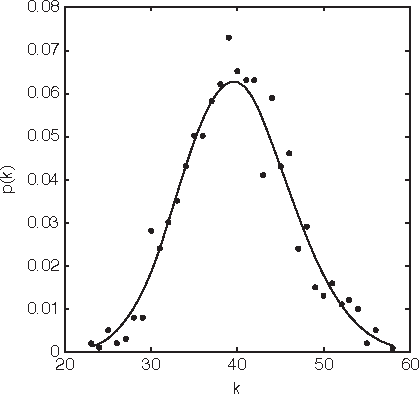
\includegraphics[height=4cm]{images/deg_dist_poisson_er.pdf}
% \end{minipage}\noindent
% \begin{minipage}[b]{0.5\textwidth}
% 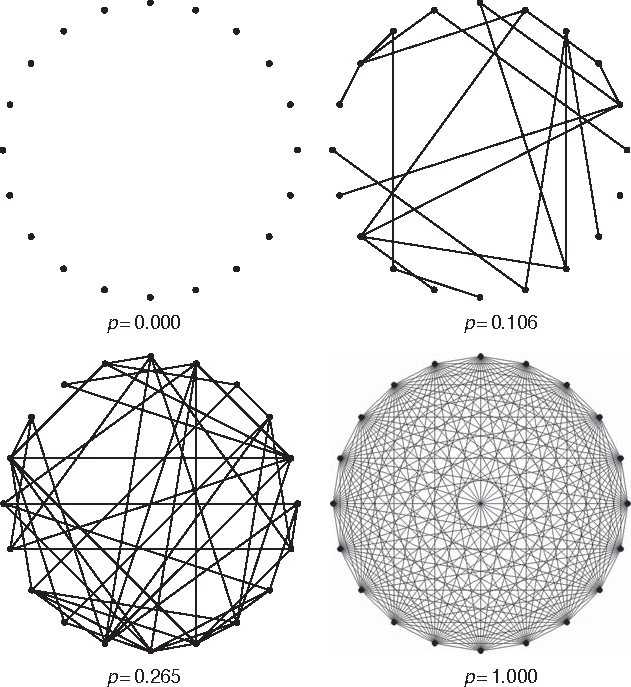
\includegraphics[height=4cm]{images/er_graphs.pdf}
% \end{minipage}
% \caption{Examples of ER graphs. On the left the Poisson degree distribution of an ER network, $n=1000$,$p=0.04$. On the right ER model instances at different values of $p$. Adapted from~\cite{Estrada2011}.}
% \label{fig:deg_dist_poisson_er}
% \end{figure}

Instead, in real networks, highly connected nodes exist within a bulk of low connected nodes and the tails of the distribution are not decaying exponentially, producing the observed phenomenon of \emph{heavy tails}.
It turns out, that many networks display a degree distribution that follows a \emph{power-law} form
\begin{equation}
\Pr(k) \propto k^{-\gamma}
\end{equation}
where $\gamma$ is usually included in the $[2,3]$ interval.
Power-law distributions, are also dubbed \emph{scale-free}, as they lack a specific scale. For some multiplicative constant $\alpha$ one indeed has that $P(\alpha k)=f(\alpha)P(k)$ where $f$ is a function only of the parameter $\alpha$. Therefore, the functional form of the power-law remain unchanged.

Hence, in understanding the limitation of the Erd\H{o}s-Rényi model, researchers developed a multitude of generative models of graphs that tried to better model properties like the heavy-tails seen in power-laws or also the \emph{small-worldness} phenomenon, i.e. the observation that most nodes in a network are reachable from every other in a small number of hops.
To keep in account the features of empirical networks, other models of networks have been developed like the models of Watts-Strogatz~\cite{Watts1998} model and Barabasi-Albert~\cite{Barabasi1999}.

For example, in the Watts-Strogatz model a graph with groups of densely connected nodes is generated as follows:
\begin{enumerate}
\item Construct a ring with $n$ nodes and connect each node to the $l$ nearest nodes ($l/2$ in each side of the ring).
\item Choose a node $i$ and the edge $e$ that connects $i$ to its nearest neighbor in a clockwise manner.
\item With probability $p_r$ replace the edge $e$ by the edge that connects $i$ to a node taken at random according to an uniform distribution over the entire ring.
\item Repeat the steps 2 and 3 for each node in clockwise manner.
\item Choose a node $i$ and the edge $e$ that connects $i$ to its second neighbor in a clockwise sense and repeat the steps 2-4.
\item Repeat the process considering the third nearest neighbor and so on, until each edge of the original lattice has been considered.
\end{enumerate}

The resulting graph shows the property of having short average path length, although the degree distribution is not power-law.
To prevent this issue, the Barabasi-Albert graph model aims to construct graphs with a dynamic attachment process.
In the BA model, one considers a small number $n_0$ of initial nodes. Then at each step, one adds a new node and connect it to a fixed number $(\leq n_0)$ of nodes that already exist in the network. The probability that the new node will be connected to a node $i$ is then proportional to $k_i^{p_s}$,  where $p_s$ is a parameter called the \emph{scaling exponent}. That algorithm generates graphs in which the frequency of nodes with degree $k$ is asymptotically proportional to ${k}^{-3}$. This power relationship between frequencies and degrees indicates that this model accounts for the power-law distribution of degrees seen in many real networks.

Although very well studied, both models are still lacking a strong community structure and more complex models have been studied by the network science community.

\section{Community detection in networks}
\label{sec:communitydetectioninnetworks}

The process of grouping nodes in a graph to establish their common behavioral properties, is a popular technique that goes under the name of \emph{community detection}. As the definition of community is not well stated, it is therefore important to have a quantitative way to evaluate the goodness of a clustering.

A \emph{quality function} is a function $\mathcal{Q}$ that given a clustering of a graph $\zeta$ returns a scalar number. Usually one identifies ``good'' clusterings with high scores of the quality function and ``bad'' clusterings with low scores. In this sense, is possible to rank partitions from bad to good, although is important to stress that the definition of ``good'' or ``bad'' is an \emph{ill-posed problem} as every quality function one designs puts the emphasis on some features of the community organization and perhaps not on others.
Here and in the following sections, we strongly point out that the concept of quality function and community detection methods are separate as the first is a way to assess the goodness of a partition while the second relies on quality function to design efficient algorithms and heuristics to find such good partitions.

One of the most important properties of a quality function is when it can be expressed as sum over communities. Such quality functions are dubbed \emph{additive}: for a generic function of a cluster $f(\zeta_i)$, an additive quality function specify the goodness of a clustering as sum of $f$ over the distinct communities as follows:
\begin{equation}\label{eq:additive_quality}
\mathcal{Q} = \sum \limits_{\zeta_c \in \zeta} f(\zeta_c).
\end{equation}
The majority of quality functions are additive, even if this requirement is not fundamental. In the next section we explore the properties of some of the most important additive quality functions that emerged from the literature of this decade.

\subsection{Spin glass based quality functions}
The simplest requirement of a quality function, is to put emphasis on intracluster edges and penalize intercluster edges. In this terms, local optima should correspond to partitions where the communities emerge as dense areas in the network loosely connected among them.
Here we present a general framework for the definition of suitable quality functions for community detection that meets these requirements.

This framework, introduced by Reichardt and Bornholdt~\cite{reichardt2006} is grounded in statistical mechanics, a branch of physics that studies the macroscopic and microscopic properties of systems of many interacting elements. Within this model, the problem of community detection is cast in terms of finding the \emph{ground state} of a spin glass, a model describing the behavior of large sets of interacting magnets.
Actually, the properties of spin glass models are subject of extremely intensive research in the last decades as their applications range from matter and nuclear physics to neural networks. Here we present only their salient application to community detection and refer the reader to cover the details of the model in other specialized books~\cite{Mezard1990}.

A spin glass model starts from the definition of an Hamiltonian, a multi-variable scalar function that describe the total energy of the physical system with the configuration of its internal components. In our case, the internal components of the system are the nodes. The configuration of the system is then expressed by the community affiliation vector $\boldsymbol\sigma$, meaning that node $i$ stays in the community $\sigma_i$ (see~\ref{sec:clustering}).
The Hamiltonian used by Reichardt and Bornholdt (RB) counts four different contributions. The first two contributions act at intracluster level, positively weighing intracluster edges and negatively weighing intracluster non-edges with coefficients $a_{ij}$ and $b_{ij}$ respectively. The third and fourth contributions work on intercluster edges and non-edges  weighing them with factors $c_{ij}$ and $d_{ij}$. The general form of the RB model is then expressed by the following Hamiltonian:

\begin{align}\label{eq:hamiltonianspinglass}
\mathcal{H}^{\textrm{RB}}(\boldsymbol \sigma) = - \sum_{(i,j)\in V^2} & \left[ a_{ij} A_{ij} - b_{ij}(1-A_{ij}) \right] \delta(\sigma_i,\sigma_j) + \nonumber \\ &  \left[ (c_{ij} A_{ij} - d_{ij}(1-A_{ij}) \right] (1-\delta(\sigma_i,\sigma_j)
\end{align}
with the convention that lowest energy states correspond to best community assignments.
Rearranging Eq.\ref{eq:hamiltonianspinglass} and discarding the terms independent of the partition into a constant $H_0$, one then gets a simpler expression for $\mathcal{H}^{\textrm{RB}}(\sigma)$:

\begin{equation}\label{eq:rbspinglass}
\mathcal{H}^{\textrm{RB}}(\boldsymbol \sigma) = -H_0 - \sum \limits_{(i,j)\in V^2} \left[ \alpha_{ij} A_{ij} - \beta_{ij} \right] \delta(\sigma_i,\sigma_j)
\end{equation}
where the two parameters $\alpha_{ij}=a_{ij}+b_{ij}+c_{ij}+d_{ij}$ and $\beta_{ij}=b_{ij}+d_{ij}$ depend on the \emph{null model} one would like to compare with, i.e. the probability that an edge exists between $i$ and $j$ after some form of edges rewiring. Hence, a null model provides a mean to compare a specific set of features of a graph, with its randomized version that should specifically lack those features.

If we get rid of the constant term $H_0$, set $\alpha_{ij}=1$ and note that the sums runs only over intracluster edges, we can express any quality function of the kind of Eq.~\ref{eq:rbspinglass} as an additive quality function, moving the summation indexes over the communities rather than over the pairs of nodes. The template Hamiltonian expressed as $\mathcal{H}^{\textrm{RB}}_{\textrm{reduced}}(\sigma)$, reads:
\begin{equation}\label{eq:rbspinglass2}
\mathcal{H}^{\textrm{RB}}_{\textrm{reduced}}(\sigma) = -\sum_{(i,j) \in V^2} \left[ A_{ij} - \beta_{ij} \right] \delta(\sigma_i,\sigma_j) = - \sum \limits_{c}^C \left[ m_c - \left< m_c \right> \right].
\end{equation}
where $m_c$ represents the number of links inside community labeled by $c$ and $\left <m_c \right >=\sum_{ij}\beta_{ij}\delta(\sigma_i,\sigma_j)$ is the expected number of links in community $c$ as prescribed by the null model $\beta_{ij}$. 
Among the additive quality functions that show up in the form of~\ref{eq:rbspinglass2}, the most important and popular is the \emph{Newman-Girvan's Modularity}.

\subsection{Newman-Girvan Modularity}
Newman-Girvan Modularity (or simply Modularity)~\cite{newman2006}, denoted here and for the rest of the work by $Q^N$, is based on the idea that a network obtained by randomly reshuffling the original graph edges while keeping the same degrees sequence, should not display any community structure. It turns out that this random reshuffling model can be computed analytically and takes the form:
\begin{equation}\label{eq:configuration_model}
\left< a_{ij} \right > = \frac{k_i k_j}{2m}
\end{equation}
where $k_i$ and $k_j$ are the degrees of node $i$ and $j$. This term of comparison (Eq.~\ref{eq:configuration}) is called ``configuration model'' and is of great importance in network science as it assigns higher probability of link to nodes with high degrees, a feature that is compatible with most real world networks.

In terms of a spin glass model, Modularity thus measures the deviation from the observed intracluster density with respect to the expected intracluster density specified by the configuration model and is described by the following equation:
\begin{equation}\label{eq:newmanmodularityspinglass}
Q^N =  \frac{1}{2m} \sum_{ (i,j) \in V^2} \left[ a_{ij} - \frac{k_i k_j}{2m} \right] \delta(\sigma_i,\sigma_j) = \sum_{c}^{C} \left[ \frac{m_c}{m} - \left( \frac{K_{\textrm{int}}(\mathcal{G}_c)}{2m} \right)^2 \right].
\end{equation}

The normalization factor $1/m$ is needed to make $Q^N$ bounded in the range $[-0.5,1]$. Modularity is an additive quality function and is relatively easy compute. Under this framework, a good partition should have $Q^N$ values close to unity, identifying groups with many more internal connections than expected at random; in contrast, a bad partition with $Q^N$ closer to zero should identify groups with no more internal connections than we expect at random.

In the next sections we will challenge this idea and show that this observation leads to false statements about modularity of networks, as a general phenomenon dubbed \emph{resolution limit}, heavily affects any quality function based on comparison with null models and specifically in the case of Newman's Modularity, hits particularly hard.

\subsection{Resolution limit in community detection}
As previously introduced, looking for 

\subsubsection{Deeper analysis of the configuration model}
In the configuration model used in Modularity the probability that a node $i$ with degree $k_i$ links any other node in the graph (including itself) is $k_i/\sum_{i}k_i$ and by means of the handshaking lemma in Eq.~\ref{eq:handshaking_lemma} is equivalent to $k_i/2m$.
Hence, in absence of correlations, is easy to show that the probability that two nodes $i$ and $j$ with degrees $k_i$ and $k_j$ are linked under this model is the product of individual probabilities:
\begin{equation}\label{eq:configuration_model_probability}
\Pr \left ( a_{ij} | \{ k \} \right) = \Pr(k_i | \{ k \})\Pr(k_j | \{ k \})=\frac{k_i k_j}{(2m)^2}
\end{equation}

Although Modularity is most frequently applied to \emph{simple graphs}( see Fig.~\ref{fig:graphmodelsa}), the configuration model implies that the randomization is carried over the space of \emph{loopy multigraphs}.
The rewiring probability considers indeed that the stubs of vertices can be reconnected both to the same source vertex (self-loops) or added to already existing edges (multi-edges).
Consider for example the set of matchings on six stubs that form a triangle graph as illustrated in Figure~\ref{fig:configuration_model_stubs}. The configuration model chooses each distinct edge stubs labeling with equal probability. However, not only the first eight distinct reshuffled labelings are possible under configuration model (Fig.\ref{fig:reshuffle_simple_graphs}) but three other distinct matchings, which produce non-simple networks (Fig.\ref{fig:reshuffle_loopy_multigraphs}). 
In fact, the number of possible rewirings that can be generated under the hypotheses of the configuration model, namely the presence of self-loops and multi-edges, is indicated by $\Omega_{CM}$ and can be computed by means of combinatorial arguments as:
\begin{equation}\label{eq:cm_possible_rewirings}
\Omega_{CM} = \binom{2m}{k_1,\ldots,k_n} = \frac{(2m)!}{\prod_i^n (k_i)!}.
\end{equation}
For the small triangle graph, this number is already very large: 90 different rewirings are possible!

In practice though, the fraction of edges involved in either self-loops or multi-edges is vanishingly small in the large $n$ limit, and thus we may generally ignore them without much impact. 
Hence, the estimate of the probability of rewiring in Eq.~\ref{eq:configuration_model_probability} is only valid in large, sufficiently sparse graphs with a sufficiently bounded degree sequence.
Under these hypotheses the expected number of edges between two vertices in the space of simple graphs is asymptotically the same as the expectation in the space of stub-labeled loopy multigraphs, i.e. the one previously introduced for the definition of Modularity: $\mathbb{E}_s[a_{ij} |k] \approx k_i k_j /(2m)$, where $s$ denotes the space of simple graphs.

% \begin{figure}[htb]
% \centering
% \begin{subfigure}[t]{0.45\textwidth}
% \centering
% 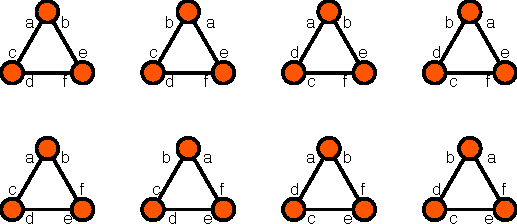
\includegraphics[width=1\textwidth]{images/configuration_model_six_stubs.pdf}
% \caption{}
% \label{fig:reshuffle_simple_graphs}
% \end{subfigure}
% \begin{subfigure}[t]{0.45\textwidth}
% 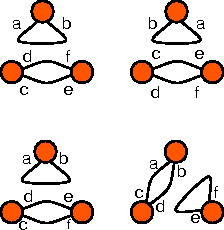
\includegraphics[width=1\textwidth]{images/configuration_model_three_stubs.pdf}
% \caption{}
% \label{fig:reshuffle_loopy_multigraphs}
% \end{subfigure}
% \caption{}
% \label{fig:configuration_model_stubs}
% \end{figure}
An approach that allows to get the right configuration model depending on the class of graph under exam relies on computational simulation of the correct rewiring probability by means of Markov Chain Monte Carlo algorithms, as proposed in ~\cite{Fosdick2016}.
In the remaining paragraphs, although flawed, we'll use the classic configuration model from Eq.~\ref{eq:configuration_model_probability} to be adherent to most of the brain networks literature, justified also by the vanishing effects of self-loops in large sparse networks. Nonetheless, we will illustrate many of the problems that the non critical use of Modularity with this null model has introduced.


Modularity identifies communities as subset of nodes whose internal fraction of edges deviates from the null configuration model on the same subset with the term $m_c/m > (K_c/2m)^2$. Despite measuring deviation from a null model, Modularity does not take into account the statistical evidence associated with this deviation and as result is not able to separate actual communities from those arising only from statistical fluctuations of the null model. Additionally, Modularity can even find high-scoring partitions in fully random graphs~\cite{Guimera2004}.

The configuration model is not the only possible null-model to use in spin-glass based quality functions and different authors proposed several variants of Modularity~\cite{ronhovde2010,ronhovde2009,traag2011} with different null models.
The simplest variation of Modularity is the so-called ER Modularity~\cite{traag2015} that instead of the configuration model uses an Erd\H{o}s-Rényi random graph in which every edge appears with the same probability $p_{ER}$. The number of expected edges $\left< m_c \right>$ in a community of size $n_c$ is thus (in the space of simple graphs):
\begin{equation}
\left< m_c \right> = p_{ER}\binom{n_c}{2}.
\end{equation}
and plugging this null model into the RB model of Eq.~\ref{eq:rbspinglass2} we obtain the model:
\begin{equation}\label{eq:ermodularityrb}
\mathcal{H}^{ER} = -\sum \limits_c^C \left[\frac{m_c}{m}  - p_{ER}\binom{n_c}{2} \right].
\end{equation}
A null model must represent some structural properties of the original graph. As the most similar ER graph of a given graph is the one that matches its density, the probability parameter $p_{ER}$ must be set equal to the original empirical graph density. We therefore obtain the so-called \emph{ER Modularity} by plugging the graph density in Eq.\ref{eq:ermodularityrb} and inverting its sign, to obtain $Q^{ER}$: 
\begin{equation}
Q^{ER} = \sum \limits_c^C \left[\frac{m_c}{m}  - \rho \binom{n_c}{2} \right].
\end{equation}
Under this model a group of nodes forms a community if its internal density is greater than the graph density $\rho$, on average.
From a machine learning perspective, one notes that all spin glass models quantify the discrepancy between observed and expected intramodule fraction of edges by means of a linear loss function.

%A common tuning to the Modularity quality function is the one that takes in consideration a \emph{resolution parameter}. From the definition of $Q^N$ is evident that is possible to tune the size of the detected modules by multiplication of the configuration null model by a constant factor $\gamma_{N} \in [0,1]$.

% Among these models, Traag et al~\cite{traag2011} takes as null model a constant quantity specified by a parameter $\gamma_{\textrm{CPM}}$.	

% The \emph{Constant Potts Model} (CPM) identifies community as subset of nodes whose internal density $\rho_c$ is bigger than the overall graph density multiplied by a factor $\gamma_{\textrm{CPM}}$ that defines the typical scale of the communities. In the framework of Reichardt and Bornholdt, the CPM model has the following Hamiltonian: 
% \begin{equation}\label{eq:cpm_hamiltonian}
% H(\sigma)^{\textrm{CPM}} = - \sum \limits_{(i,j) \in V^2} \left[ a_{ij} - \rho \gamma_{\textrm{CPM}} \right] \delta(\sigma_i,\sigma_j).
% \end{equation}
% Reworking~\ref{eq:cpm_hamiltonian} and using the definitions of intracluster edges and intracluster nodes one can write the model is simple terms as
% \begin{equation}\label{eq:cpm_ermodel}
% H(\sigma)^{\textrm{CPM}} = - \sum \limits_c^C \left[m_c - \gamma_{\textrm{CPM}} n_c^2 \right] 
% \end{equation}
% In other words, the model tries to maximize the number of internal edges while at the same time keeping relatively small communities. The parameter $\gamma_{\textrm{CPM}}$ balances these two imperatives. In fact, the parameter $\gamma_{\textrm{CPM}}$ acts as the inner and outer edge density threshold. That is, suppose there is a community c with $m_c$ edges and $n_c$ nodes. Then is better to split it into two communities $r$ and $s$ if: 
% \begin{equation}
% \frac{m_{r,s}}{2n_r n_s} < \gamma_{\textrm{CPM}}
% \end{equation}

\subsubsection{Surprise}\label{sec:surprise}

Comparison with the graph density is part of the idea that led to a definition of a different kind of quality function that is not additive nor is based on a spin glass model but rather relies on statistical bases. In comparing the fraction of edges falling within modules against another expected value one is indeed making a statistical test to validate the hypothesis that the two populations are from the same distribution. To which level of statistical significance this test is valid though is not answered by none of the spin glass based functions.


% \section{Artificial functional connectivity pipeline}\label{sec:artificialpipeline}
% pipeline
% \section{Quality functions}
% 	\subsection{Newman modularity}
% 	\subsection{Surprise}
% 	\subsection{Asymptotical Surprise}
% 	\subsection{Infomap}

% 	\section{Optimization methods}
% 	\subsection{Louvain}
% 	\subsection{Infomap}
% 	\subsection{FAGSO}
% 	\subsection{PACO}

% \section{Measuring partition similarity}
% 	\subsection{Information theory based}
% 	\subsection{NMI}
% 	\subsubsection{VI}
% 	\subsection{Correction for randomness: rNMI}

% 	\subsection{Sensitivity-specificity}

% 	\section{Benchmark networks}
% 	\subsection{Ring of cliques}
% 	\subsection{Stochastic block models}
% 	\subsection{Unweighted LFR}
% 	\subsection{Weighted LFR}
% 	\subsection{Covariate LFR}


%%%%%%%%%%%%%%% TRASH %%%%%%%%%%%%%%%%%%%%%
% \begin{figure}[htb]
% \centering
% \begin{tabular*}{0.85\textwidth}{l @{\extracolsep{\fill}} l @{\extracolsep{\fill}} l}
% {\Large{\textsf A.}} & {\Large{\textsf B.}} & {\Large{\textsf C.}}\\
% \begin{tikzpicture}
% 	\GraphInit[vstyle=Normal]
% 	\SetGraphUnit{1.5}
% 	\begin{scope}[rotate=-135]
% 	\Vertices{circle}{a,b,c,e}
% 	\end{scope}
% 	\NOEA[unit=1.414](e){d}
% 	\Edges(a,b,e,d,c,e,a,c,b)
% \end{tikzpicture}
% &
% \begin{tikzpicture}
% 	\tikzset{LabelStyle/.style= {draw}}
% 	\GraphInit[vstyle=Normal]
% 	\SetGraphUnit{1.5}
% 	\begin{scope}[rotate=-135]
% 	\Vertices{circle}{a,b,c,e}
% 	\end{scope}
% 	\NOEA[unit=1.414](e){d}
% 	\Edge[label=1](a)(b)
% 	\Edge[label=2](a)(c)
% 	\Edge[label=4](a)(b)
% 	\Edge[label=0.5](d)(e)
% 	\Edge[label=0.25](d)(c)
% 	\Edge[label=0.15](c)(b)
% 	\Edge[label=0.45](e)(a)
% 	\Edge[label=3](e)(c)
% 	\Edge[label=6](e)(b)
% 	\Edge (a)(d)
% \end{tikzpicture}
% &
% \begin{tikzpicture}
% 	\GraphInit[vstyle=Normal]
% 	\SetGraphUnit{1.5}
% 	\begin{scope}[rotate=-135]
% 	\Vertices{circle}{a,b,c,e}
% 	\end{scope}
% 	\NOEA[unit=1.2](e){d}
% 	\Edges(a,b,c,d,e)
% 	\Loop[dist = 1.5cm, dir = SO](d)
% 	\tikzset{EdgeStyle/.append style = {bend right = 15}}
% 	\Edge(c)(b)
% 	\Edge(e)(a)
% 	\tikzset{EdgeStyle/.append style = {bend left = 15}}
% 	\Edge(c)(b)
% 	\Edge(a)(b)
% 	\tikzset{EdgeStyle/.append style = {bend left = 30}}
% 	\Edge(c)(b)
% 	\Edge(e)(a)
% 	\tikzset{EdgeStyle/.append style = {bend right = 30}}
% 	\Edge(c)(b)
% \end{tikzpicture}
% \end{tabular*}
% \caption{Three models of graphs. (A) Simple unweighted graph. Simple edge-weighted graph. (C) Graph with multiedges and self-loops.}
% \label{fig:graphmodels}
% \end{figure}